\subsubsubsubsection{Urban entity builder}
\begin{figure}[h]
\centering
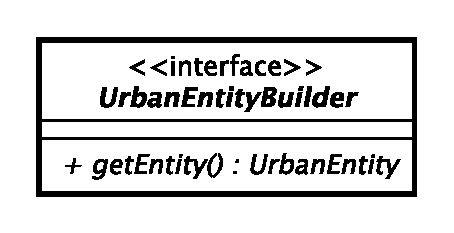
\includegraphics[scale=0.6,keepaspectratio]{images/solution/app/backend/urban_entity_builder.eps}
\caption{\pReactiveBuild::UrbanEntityBuilder}
\label{fig:sd-app-UrbanEntitybuilder}
\end{figure}
\FloatBarrier
\begin{itemize}
  \item \textbf{\descr} \\
    It represents a component that builds urban entities like crossroads and
    streets.
  \item \textbf{\ops}
  \begin{itemize}
    \item[+] \texttt{\textit{getEntity() : UrbanEntity}} \\
Returns the final product of the building.
  \end{itemize}
\end{itemize}
